\chapter{Einleitung}

Dies ist die Einleitung.

Lorem ipsum dolor sit amet, consectetur adipiscing elit. Sed gravida mollis placerat. Sed congue iaculis massa vitae dapibus. Fusce sed felis lorem. Suspendisse purus diam, sollicitudin vitae imperdiet ac, placerat eu metus. In luctus, metus vel dictum hendrerit, diam lacus cursus enim, eu porta augue lacus non metus. Pellentesque habitant morbi tristique senectus et netus et malesuada fames ac turpis egestas. Nullam nec orci eget metus pulvinar sagittis. Vestibulum ante ipsum primis in faucibus orci luctus et ultrices posuere cubilia Curae; Sed turpis lorem, aliquet eu ornare non, viverra ac urna.

\section{Big Picture}

\begin{flushleft}
Zur Übersicht wird das Umfeld der Applikation in einem Big Picture zusammengefasst.
Die Darstellung wird in drei Abschnitte uterteilt. Im obersten Abschnitt befinden sich alle Geräte, welche Daten liefern. Diese sind alle Android Aufnahmesysteme, welche in dieser Arbeit umgesetzt werden, sowie der RadioTourSpeaker, welcher bereits vorhanden ist. \linebreak 
Im mittleren Teil befindet sich die Serverseite. Diese besteht aus einem TourLiveServer, welcher alle Renndaten sammelt und einem Devicemanagement Server, welcher die Einstellungen aller Aufnahmesysteme speichert und die Möglichkeit bietet, diese zu bearbeiten.\linebreak 
Der unterste Abschnitt zeigt Beispiele von Parteien, die mit den Daten beliefert werden. Dies kann die Webseite sein, die in dieser Arbeit umgesetzt wird, jedoch auch Drittanbieter, die Interesse an diesen Daten haben.

\end{flushleft}
\begin{figure}[H]
	\centering
	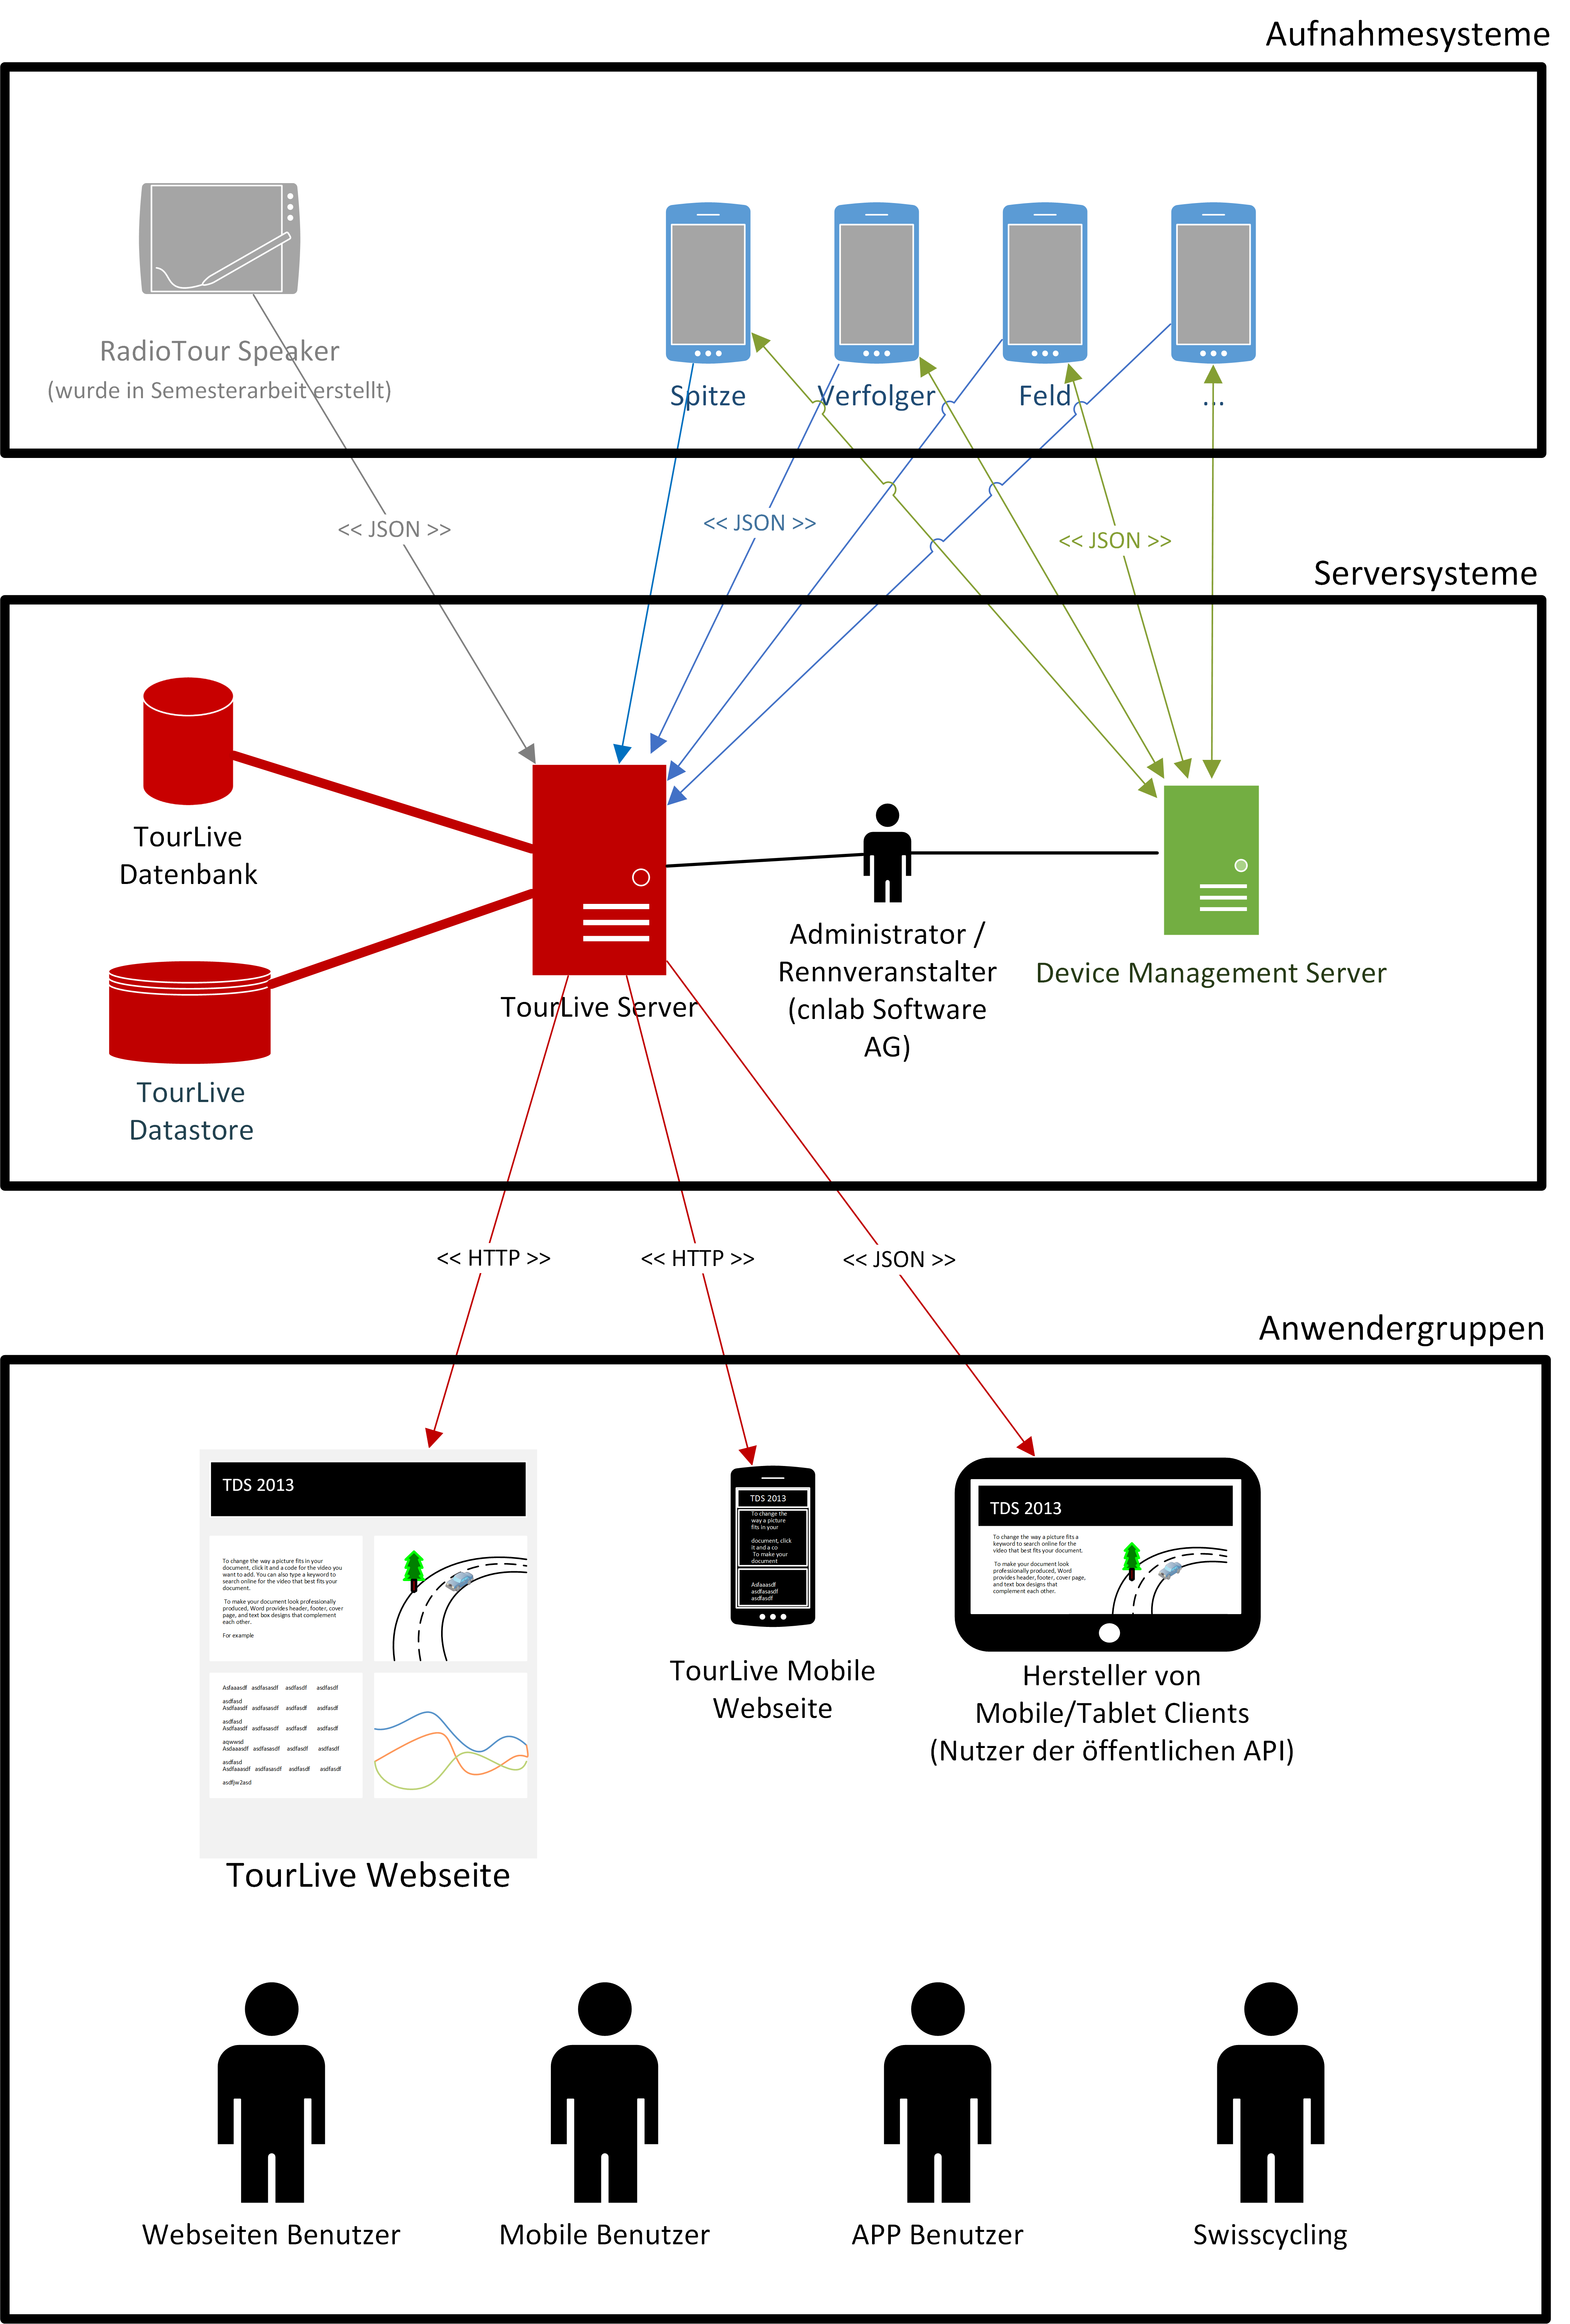
\includegraphics[height=200mm]{images/BigPicture.png}
	\caption{BigPicture}
\end{figure}

\section{Aufgabenteilung}

Lorem ipsum dolor sit amet, consectetur adipiscing elit. Sed gravida mollis placerat. Sed congue iaculis massa vitae dapibus. Fusce sed felis lorem. Suspendisse purus diam, sollicitudin vitae imperdiet ac, placerat eu metus. In luctus, metus vel dictum hendrerit, diam lacus cursus enim, eu porta augue lacus non metus. Pellentesque habitant morbi tristique senectus et netus et malesuada fames ac turpis egestas. Nullam nec orci eget metus pulvinar sagittis. Vestibulum ante ipsum primis in faucibus orci luctus et ultrices posuere cubilia Curae; Sed turpis lorem, aliquet eu ornare non, viverra ac urna.